% Metódy inžinierskej práce

\documentclass[10pt,twoside,slovak,a4paper]{coursepaper}

\usepackage[slovak]{babel}
%\usepackage[T1]{fontenc}
\usepackage[IL2]{fontenc} % lepšia sadzba písmena Ľ než v T1
\usepackage[utf8]{inputenc}
\usepackage{graphicx}
\usepackage{url} % príkaz \url na formátovanie URL
\usepackage{hyperref} % odkazy v texte budú aktívne (pri niektorých triedach dokumentov spôsobuje posun textu)

\usepackage{cite}
%\usepackage{times}

\pagestyle{headings}

\title{Evolúcia počítaťových hier\thanks{Semestrálny projekt v predmete Metódy inžinierskej práce, ak. rok 2022/23, vedenie: Dávid Babiš}} % meno a priezvisko vyučujúceho na cvičeniach

\author{Dávid Babiš\\[2pt]
	{\small Slovenská technická univerzita v Bratislave}\\
	{\small Fakulta informatiky a informačných technológií}\\
	{\small \texttt{xbabis@stuba.sk}}
	}

\date{\small 30. marec 2003} % upravte



\begin{document}

\maketitle

\begin{abstract}
To, že sa počítačové hry z roka na rok menia a vylepšujú, nie je pre vás určite novinkou. Vidieť ju však v rozmedzí mnoho rokov je zaručene niečo neopísateľné. Počítačová technika ide neuveriteľne rýchlo dopredu. Tieto hry sú s nami iba pár desiatok rokov, ale za tú dobu sa stihli výrazne zmeniť. Od jednoduchých pixelov na čiernobielych monitoroch sme sa dostali k prepracovanej grafike, ktorá nielen verne zachytáva našu skutočnosť, ale dokáže vykresliť aj neskutočnosť. Napríklad fantastické svety ktoré existujú len vo videohrách.  V tomto článku sa dozviete, ako sa menila nielen grafická stránka počítačových hier od roku 1952. Rozdiel je naozaj obrovský. Pamätáte si ešte niektoré staré klasiky?
\end{abstract}



\section{Úvod}
 Od jednoduchých pixelov na čiernobielych monitoroch sme sa dostali k prepracovanej grafike, ktorá nielen verne zachytáva našu skutočnosť, ale dokáže vykresliť aj neskutočnosť. Napríklad fantastické svety ktoré existujú len vo videohrách.  V tomto článku sa dozviete, ako sa menila nielen grafická stránka počítačových hier od roku 1952. Rozdiel je naozaj obrovský. Pamätáte si ešte niektoré staré klasiky?
Motivujte čitateľa a vysvetlite, o čom píšete. Úvod sa väčšinou nedelí na časti.
Uveďte explicitne štruktúru článku. Tu je nejaký príklad.
Základný problém, ktorý bol naznačený v úvode, je podrobnejšie vysvetlený v časti~\ref{nejaka}.
Dôležité súvislosti sú uvedené v častiach~\ref{dolezita} a~\ref{dolezitejsia}.
Záverečné poznámky prináša časť~\ref{zaver}.

\section{História}

\subsection{NIMROD 1951}
V roku 1951 bol pri príležitosti "Festival of Britain" predstavený digitálny počítač Ferranti NIMROD. Išlo o prvý počítač navrhnutý špeciálne pre počítačovú hru. Tento stroj so spotrebou krásnych 6 kilowattov a frekvenciou procesora 10kHz vedel, ako už názov napovedá, jedinú hru - NIM. Pôvodom pravdepodobne v Číne, NIM je jednoduchá logická hra pre dvoch hráčov spočívajúca v odoberaní prvkov z niekoľkých (typicky troch) množín. V každom ťahu môže hráč odobrať ľubovoľné množstvo prvkov (miniálne jeden) z jednej množiny. Víťazom je ten hráč, ktorý odoberie posledný prvok.

Ako „grafický“ výstup bol použitý panel so žiarovkami. NIMROD teda nie je mnohými považovaný za skutočnú videohru, pretože nepoužíva zobrazovacie zariadenie typu TV/monitor a pod. Ale to sa zase dostávame k problematickej definícii videohry. O niečo neskôr bol NIMROD s veľkým úspechom vystavený aj v Berlíne.
\subsection{OXO 1952} \label{nejaka}
Za prvú skutočnú videohru je možné OXO považovať najmä preto, že pre jej grafický výstup bola vôbec prvýkrát v dejinách počítačov použitá osciloskopická obrazovka, teda monitor.Vznikla v roku 1952.  Zobrazenie bitmapy bolo 35 × 16 pixelov. Hra bola nainštalovaná na elektrónkovom počítači EDSAC, ktorý bežne používal dierne pásky. Zahrať ste si mohli jedine proti umelej inteligencii. Ovládať ju bolo možné pomocou vytáčacieho telefónu, pričom vytočené číslo znamenalo políčko, na ktoré hráč umiestnil guľôčku alebo krížik.
Hra bola na počítači EDSAC nainštalovaná iba po dobu Douglesovej dizertačnej práce a širokej verejnosti sprístupnená nikdy nebola. Po obhájení svojej práce musel Douglles hru z počítača vymazať, pretože zaberala príliš mnoho miesta. 

Z obr.~\ref{f:rozhod} je všetko jasné. 

\begin{figure*}[tbh]
\centering
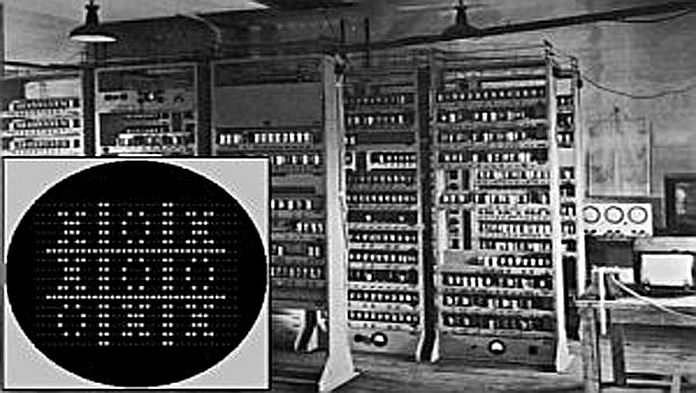
\includegraphics[scale=0.5]{Schránka-15.jpg}
%Aj text môže byť prezentovaný ako obrázok. Stane sa z neho označný plávajúci objekt. Po vytvorení diagramu zrušte znak \texttt{\%} pred príkazom \verb|\includegraphics| označte tento riadok ako komentár (tiež pomocou znaku \texttt{\%}).
\caption{Rozhodujúci argument.}
\label{f:rozhod}
\end{figure*}



\section{Iná časť} \label{ina}

Základným problémom je teda\ldots{} Najprv sa pozrieme na nejaké vysvetlenie (časť~\ref{ina:nejake}), a potom na ešte nejaké (časť~\ref{ina:nejake}).\footnote{Niekedy môžete potrebovať aj poznámku pod čiarou.}

Môže sa zdať, že problém vlastne nejestvuje\cite{Coplien:MPD}, ale bolo dokázané, že to tak nie je~\cite{Czarnecki:Staged, Czarnecki:Progress}. Napriek tomu, aj dnes na webe narazíme na všelijaké pochybné názory\cite{PLP-Framework}. Dôležité veci možno \emph{zdôrazniť kurzívou}.


\subsection{Nejaké vysvetlenie} \label{ina:nejake}

Niekedy treba uviesť zoznam:

\begin{itemize}
\item jedna vec
\item druhá vec
	\begin{itemize}
	\item x
	\item y
	\end{itemize}
\end{itemize}

Ten istý zoznam, len číslovaný:

\begin{enumerate}
\item jedna vec
\item druhá vec
	\begin{enumerate}
	\item x
	\item y
	\end{enumerate}
\end{enumerate}


\subsection{Ešte nejaké vysvetlenie} \label{ina:este}

\paragraph{Veľmi dôležitá poznámka.}
Niekedy je potrebné nadpisom označiť odsek. Text pokračuje hneď za nadpisom.



\section{Dôležitá časť} \label{dolezita}




\section{Ešte dôležitejšia časť} \label{dolezitejsia}




\section{Záver} \label{zaver} % prípadne iný variant názvu


%\input{example.tex}



%\acknowledgement{Ak niekomu chcete poďakovať\ldots}


% týmto sa generuje zoznam literatúry z obsahu súboru literatura.bib podľa toho, na čo sa v článku odkazujete
\bibliography{literatura}
\bibliographystyle{alpha} % prípadne alpha, abbrv alebo hociktorý iný
\end{document}
